\section{Описание работы}
Подготовить исходные данные с помощью программы Avogadro. Провести расчетов в одной точке (Single Point Caclucation) и оптимизация геометрии (Energy Optimization) с помощью программы GAMESS. Проанализировать результаты.

Расчитываемая молекула: изопропанол $CH_3 - CHOH - CH_3$
\begin{figure}[H]
\centering
\captionsetup{justification=centering}
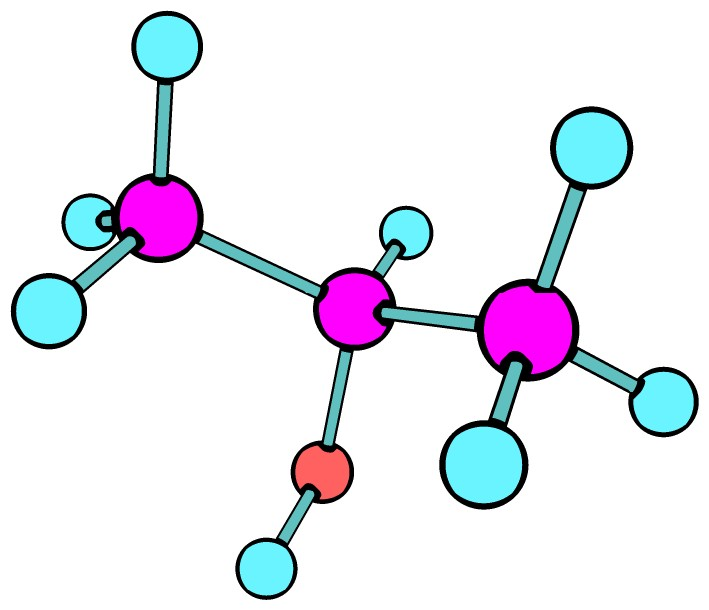
\includegraphics[scale=0.4]{fig/0.jpg}
\caption{Изопропанол. Цветами обозначены атомы: голубой - водород, фиолетовый - углерод, красный - кислород.}
\end{figure}

Приложенные файлы:
\begin{itemize}
    \item structure.cml – файл исходных данных;
    \item Isopropanol\_6-31G.inp – исходные данные GAMESS для расчета методом RHF в базисе6-31G;
    \item Isopropanol\_6-31G.log – результат расчета методом RHF в базисе 6-31G;
    \item Isopropanol\_6-31G+dp.inp – исходные данные GAMESS для расчета методом RHF в базисе 6-31G+(d, p);
    \item Isopropanol\_6-31G+dp.log – результат расчета методом RHF в базисе 6-31G+(d, p);
    \item Isopropanol\_opt\_es\_6-31G.inp - исходные данные GAMESS для расчета методом RHF в базисе 6-31G с оптимизацией геометрии до ES;
    \item Isopropanol\_opt\_es\_6-31G.log - результат расчета методом RHF в базисе 6-31G с оптимизацией геометрии до ES.
\end{itemize}{}

\section{Постановка задачи}
Предварительно оптимизировать молекулярную структуру с помощью программы AVOGADRO, затем провести геометрическую оптимизацию с помощью программы GAMESS с помощью метода RHF. Затем проанализировать следующие показатели: 
\begin{itemize}
    \item количество заполненных МО; 
    \item номер слейтеровской орбитали, локализованной на атоме кислорода, которая вносит существенный вклад в HOMO;
    \item для 1-го расчета определить заселенность по Малликену атома кислорода;
    \item наибольшие по величине элементы матрицы плотности, из числа относящихся к паре атомов OH, соединенных ковалентной связью;
    \item для 2-го расчета сравнить полученную полную энергию (в а.е.) с энергией, полученной в 1-м расчете;
    \item для 3-го расчета (с оптимизацией геометрии до ES) привести исходное значение полной энергии (в а.е.) до начала процесса оптимизации и полную энергию, полученную после завершения процесса оптимизации геометрии. Для полной энергии, полученной по окончанию оптимизации, привести вклады электронной энергии и энергии кулоновского отталкивания ядер.
    \item для 3-го расчета сопоставить геометрии (длины связей) до и после оптимизации методом Хартри-Фока, визуализировать результат оптимизации с помощью программы Avogadro.
\end{itemize}

\newpage
\section{Теоретическая информация}
\subsection{Ограниченный метод Хартри-Фока}
В методе Хартри-Фока волновая функция приближенно описывается одним детерминантов Слэтера, параметры которого оптимизируют согласно вариационному принципу:\par\textit{
Для любого $\Psi$, удовлетворяющего условию нормировки $\braket{\Psi|\Psi} = 1$ выполняется соотношение $\braket{\Psi|\hat{H}|\Psi} \geq E_0$, где $E_0$ - энергия основного состояния системы, описываемого гамильтонианом $\hat{H}$}

Метод ХФ называют моделью "независимых электронов": предполагается, что каждый электрон движется в некотором поле, создаваемом другими электронами и ядрами, и вместе эти поля образуют некоторое эффективное среднее поле\footnote{Поскольку каждый электрон влияет на движение окружающих электронов и в то же этом находится под их влиянием, то результирующее поле также называют \textit{самосогласованным}.}. В методе каждому электрону сопоставляется одна спин-орбиталь и оптимизируют параметры этих спин-орбиталей. 

Одной из версий метода Хартри-Фока, применяемый для описания синглетных состояний систем с замкнутой оболочкой, является \textit{ограниченный метод ХФ (RHF)}. Метод предполагает двукратное заполнение пространственных орбиталей электронами с разной проекцией спина.

\subsection{Метод Хартри-Фока-Рутана}
Уравнение Хартри-Фока представляет собой систему связанных интегро-дифференциальных уравнений. При рассмотрении молекулярных систем решение системы уравнений аппроксимируют линейной комбинацией некоторых заранее определенных базисных функций. Базисные орбитали обычно центрированы на разных атомах, и виды этих базисных функций берут из расчетов свободных атомов. Поэтому метод Хартри-Фока-Рутана также называют подходом аппроксимации \textit{молекулярных орбиталей как линейной комбинации атомных орбиталей (МО-ЛКАО)}.

\subsection{Анализ заселенностей}
Электронную плотность в точке $\Vec{r}$ можно рассматривать как среднее значение оператора $\hat{\rho}(\Vec{r})$, имеющего вид:
\begin{equation}\label{eq:1}
    \hat{\rho}(\Vec{r}) = \sum\limits_{i=1}^n \delta(\Vec{r} - \Vec{r_i})
\end{equation}{}

Если многоэлектронная волновая функция является детерминантом Слетера, построенным из ортонормированных спион-орбиталей, то среднее значение электронной плотность можно вычислить следующим образом:
\begin{equation}\label{eq:2}
    \rho(\Vec{r}) = \braket{\Psi|\sum\limits_{j=1}^n \delta(\Vec{r} - \Vec{r_j})|\Psi} = \sum\limits_{i=1}^n\braket{\psi_i(\Vec{r_1}, \sigma_1)|\delta(\Vec{r} - \Vec{r_1})|\psi_i(\Vec{r_1}, \sigma_1)} = \sum\limits_{i=1}^{n_\alpha}|\psi_i^\alpha(\Vec{r})|^2 + \sum\limits_{i=1}^{n_\beta}|\psi_i^\beta(\Vec{r})|^2
\end{equation}
Здесь суммирование идет по $n_\alpha$ молекулярным орбиталям, занятых электронами с проекцией спина $\alpha$, и по $n_\beta$ молекулярным орбиталям, занятых электронами с проекцией спина $\beta$. 

Если использовать разложение МО-ЛКАО, то электронную плотность можно выразить через набор атомных орбиталей $\{\chi(\Vec{r})\}_{i=1}^{m}$:
\begin{equation}
\begin{split}
\begin{gathered}
    \rho(\Vec{r}) =  
    \sum\limits_{i=1}^{n_\alpha}\psi_i^{\alpha*}(\Vec{r})\psi_i^{\alpha}(\Vec{r}) + \sum\limits_{i=1}^{n_\beta}\psi_i^{\beta*}(\Vec{r})\psi_i^{\beta}(\Vec{r}) 
    = 
    \sum\limits_{i=1}^{n_\alpha}\sum\limits_{\mu=1}^{m}c_{i\mu}^{\alpha*}\chi_\mu^{*}\sum\limits_{\nu=1}^{m}c_{i\nu}^{\alpha}\chi_\nu +
    \sum\limits_{i=1}^{n_\beta}\sum\limits_{\mu=1}^{m}c_{i\mu}^{\beta*}\chi_\mu^{*}\sum\limits_{\nu=1}^{m}c_{i\nu}^{\beta}\chi_\nu = \\ 
    =
    \sum\limits_{\mu,\nu=1}^{m}(P_{\mu\nu}^{\alpha} + P_{\mu\nu}^{\beta})\chi_\mu^{*}\chi_\nu 
    = 
    \sum\limits_{\mu,\nu=1}^{m}D_{\mu\nu}\chi_\mu^{*}\chi_\nu
\end{gathered}
\end{split}
\end{equation}

Здесь введен $\textbf{P}$ -- спиновая матрица плотности, элементы которой определены следующим образом:
\begin{equation}
    P_{\mu\nu}^\alpha = \sum\limits_{i=1}^{n_\alpha}c_{i\mu}^{\alpha*}c_{i\nu}^{\alpha}
\end{equation}

$\textbf{D}$ - бесспиновая матрица плотности, определенная как:
\begin{equation}
    \textbf{D} = \textbf{P}^{\alpha} + \textbf{P}^{\beta}
\end{equation}

Если проинтегрировать электронную плотность по всему объему, то получится полное число электронов $n = n_\alpha + n_\beta$:

\begin{equation}
    n = \sum\limits_{\nu,\mu=1}^{m}D_{\mu\nu}S_{\nu\mu}
\end{equation}

Величину
\begin{equation}
    q_{\mu} = \sum\limits_{\nu=1}^{m}D_{\mu\nu}S_{\nu\mu}
\end{equation}
называют \textit{полной орбитальной заселенностью по Малликену} базисной орбитали $\chi_{\mu}$. Формально можно разбить данную величину на два терма:

\begin{equation}
    q_{\mu} = D_{\mu\mu} + \sum\limits_{\substack{\nu=1 \\ \nu\neq\mu}}^{m}D_{\mu\nu}S_{\nu\mu}
\end{equation}

Первый терм называют \textit{чистой орбитальной заселенностью по Малликену} орбитали $\chi_\mu$. Можно заметить, что во втором терме в случае вещественности базисных функций справедливо $D_{\mu\nu}S_{\nu\mu} = D_{\nu\mu}S_{\mu\nu}$, тогда величину
$2D_{\mu\nu}S_{\nu\mu}$ называют \textit{заселеленностью перекрывания} между орбиталями $\chi_\mu$ и $\chi_\nu$.

Чтобы получить \textit{полную атомную заселенность} на атоме $A$, необходимо просуммировать по всем атомным орбиталям, центрированным на данном атоме:
\begin{equation}
    Q_{A} = \sum\limits_{\mu\in A}q_{\mu} = \sum\limits_{\mu\in A}\sum\limits_{\nu=1}^{m}D_{\mu\nu}S_{\nu\mu}
\end{equation}

Похожим образом можно ввести понятия \textit{чистой атомной заселенности} и \textit{атомной заселенности перекрывания}:
\begin{equation}
    Q_{A} = \sum\limits_{\mu\in A}\sum\limits_{\nu=1}^{m}D_{\mu\nu}S_{\nu\mu} = \sum\limits_{\mu, \nu \in A}D_{\mu\nu}S_{\nu\mu} + \sum\limits_{\mu\in A}\sum\limits_{\nu\in B}D_{\mu\nu}S_{\nu\mu} = d_{A} + \sum\limits_{\substack{B \\ B \neq A}}d_{AB}
\end{equation}

Как и в случае с орбитальной заселенностью, в случае вещественности базисных функций величину $d_{AB} + d_{BA} = 2d_{AB}$ называют \textit{атомной заселенности перекрывания}.

\newpage
\section{Результаты}
\subsubsection*{Сколько МО заполнено у данной молекулы?}
17 полностью заполненных пространственных МО (раздел NUMBER OF OCCUPIED ORBITALS).

\subsubsection*{Определить номер HOMO, которая содержит существенный вклад АО, локализованной на атоме кислорода.}
Номер HOMO 17. Наиболее существенный вклад вносит $2p_x$-орбиталь, 0.494465 (раздел EIGENVECTORS).

\subsubsection*{Определить заселенность по Малликену атома кислорода}
8.7. Так как заряд ядра атома кислорода составялет +8, то в данном соединении кислород является электроотрицательным (раздел TOTAL MULLIKEN AND LOWDIN ATOMIC POPULATIONS).

\subsubsection*{Анализ связи OH}
\begin{figure}[H]
\centering
\captionsetup{justification=centering}
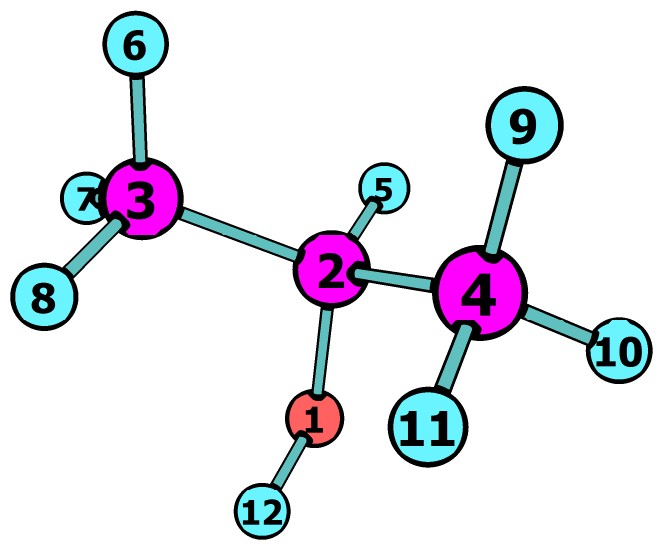
\includegraphics[scale=0.4]{fig/1.jpg}
\caption{Номера атомов в молекуле изопропанола. Цветами обозначены атомы: голубой - водород, фиолетовый - углерод, красный - кислород.}
\end{figure}

Наибольшие по величине элементы матрицы плотности:
\begin{equation}
\begin{split}
\begin{gathered}
D_{51,2} = 0.073202 \\
D_{51,6} = 0.047307 \\
D_{52,1} = 0.017844
\end{gathered}
\end{split}
\end{equation}

Межатомная заселенность по Малликену составялет 0.511622 (разделы DENSITY MATRIX, MULLIKEN ATOMIC OVERLAP POPULATIONS).

\subsubsection*{Сравнение результатов расчетов различных базисов}
Полная энергия системы, рассчитанной методом RHF в базисе 6-31G, равна -193.03 Хартри. Для системы, рассчитанной в базисе 6-31G+(d,p)\footnote{Символ '+' значит, что к базисному набору добавляются диффузионные функции (d-функции) для всех тяжелых атомов, а (d,p) - добавляются поляризационные функции (p-функции) для всех атомов.} -- -193.13 Хартри. 

Делать какой-либо вывод о качестве схем расчета только на основании знаний полной энергии некорректно. Качество и корректность используемых схем расчета мы можем оценить, сопоставив теоретически полученные результаты с экспериментальными. То есть мы должны исследовать конкретный физический процесс: например это могло быть определение энергии диссоциации молекулы.

Однако чем большим количеством функций мы аппроксимируем вид волновой функции системы, тем ближе результат к истинному: если  число базисных функций стремится к полному $m \rightarrow \infty$, то использование метода МО-ЛКАО эквивалентно точному решению уравнения Шрёдингера. А это значит, что и параметры системы, определяемые волновой функцией, также становятся точнее. Проведенные расчеты подтверждают это\footnote{Напомню, что согласно вариационное принципу система, описываемая гамильтонианом $\hat{H}$, в основном состоянии достигает минимума энергии.}
(разделы ENERGY COMPONENTS до и после оптимизации).

\subsubsection*{Оптимизация геометрии. Сопоставление полной энергии}
Была проведена оптимизация геометрии методом RHF в базисе 6-31G.

\begin{table}[H]
\caption{Значения составляющих полной энергии для молекулы до и после проведения оптимизации (в Хартри)} \label{tab:my-table}
    \begin{center}
        \begin{tabular}{|c|c|c|}
        \hline
         & До оптимизация & После оптимизации \\ \hline
        \begin{tabular}[c]{@{}c@{}}Кинетическая энергия\\ электронов\end{tabular} & 193.182 & 193.266 \\ \hline
        \begin{tabular}[c]{@{}c@{}}Электрон-электронное\\ взаимодействие\end{tabular} & 201.331 & 200.848 \\ \hline
        \begin{tabular}[c]{@{}c@{}}Электрон-ядерное\\ взаимодействие\end{tabular} & -722.645 & -721.726 \\ \hline
        \begin{tabular}[c]{@{}c@{}}Ядер-ядерное\\ взаимодействие\end{tabular} & 135.097 & 134.575 \\ \hline
        \textbf{Полная энергия} & \textbf{-193.034} & \textbf{-193.036} \\ \hline
        \end{tabular}
    \end{center}
\end{table}

Изменение полной энергии составило менее 1\%, что является несущественным. Это значит, что Авогадро хорошо проводит оптимизацию.

\newpage
\subsubsection*{Оптимизация геометрии. Сопоставление длин связей}
Была проведена оптимизация геометрии методом RHF в базисе 6-31G.

\begin{figure}[H]
\centering
\captionsetup{justification=centering}
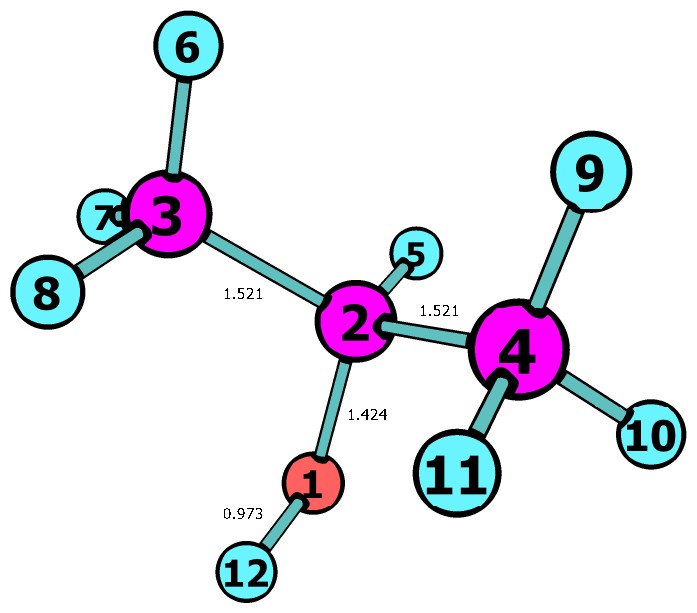
\includegraphics[scale=0.4]{fig/2.jpg}
\caption{Геометрия молекулы до оптимизации}
\end{figure}

\begin{figure}[H]
\centering
\captionsetup{justification=centering}
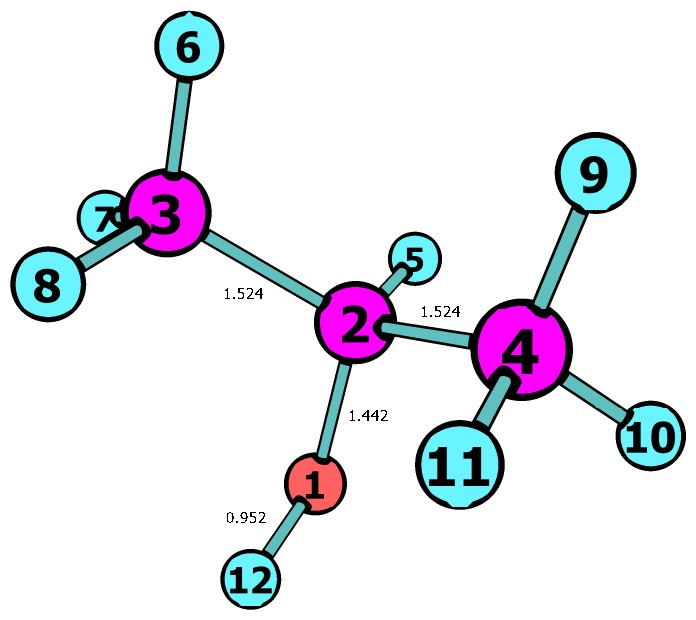
\includegraphics[scale=0.4]{fig/3.jpg}
\caption{Геометрия молекулы после оптимизации}
\end{figure}

Как видно из рисунков, наиболее существенно изменилась длина связи O1-H12 \\ ($\Delta = 0.021$\AA, $\approx2\%$).

\newpage
\section{Контроль результатов}
\begin{enumerate}
    \item Поскольку 1-й и 2-й расчеты проведены в одной и той же геометрии, они отличаются только по величине электронной энергии. Вклад энергии межъядерного отталкивания один и тот же.
    \item При сопоставлении 1-го и 2-го расчетов действительно оказывается, что расчет, проведенный в более широком базисе дает более точную полную энергию.
    \item Процесс оптимизации геометрии в 3-ем расчете действительно завершен (в выходном файле содержится ''EQUILIBRIUM GEOMETRY LOCATED''). В результате 3-го расчета (по завершению процесса оптимизации геометрии) получена более низкая полная энергия, чем в 1-м расчете.
\end{enumerate}{}